% =========================================================
% multilingual_llm_review.tex
% ACM Computing Surveys-style review paper
% =========================================================

\documentclass[acmsmall,screen,review]{acmart}

\setcopyright{none}
\settopmatter{printacmref=false}
\renewcommand\footnotetextcopyrightpermission[1]{}

\ccsdesc[500]{Computing methodologies~Natural language processing}
\ccsdesc[300]{Information systems~Digital libraries and archives}
\ccsdesc[300]{Computing methodologies~Machine learning}

\acmJournal{CSUR}

\usepackage{booktabs}
\usepackage{tabularx}
\usepackage{array}
\usepackage{multirow}
\usepackage{graphicx}

% ---------------------------------------------------------
% TITLE
% ---------------------------------------------------------

\title[Multilingual Reliability of LLMs]
{Evaluating Multilingual Reliability of Large Language Models in Scientific Literature Analysis}

\subtitle
{A Review of Cross-Lingual Factuality, Hallucination, and Benchmarking Approaches for LLM-Assisted Scientific Text Analysis}

% ---------------------------------------------------------
% AUTHOR DETAILS
% ---------------------------------------------------------

\author{Prakhar Srivastava}

\affiliation{%
  \institution{Department of Information Technology, IIIT Allahabad}
  \country{India}
}

\email{pns2026002@iiita.ac.in}

\renewcommand{\shortauthors}{Prakhar Srivastava}

% ---------------------------------------------------------
% ABSTRACT
% ---------------------------------------------------------

\begin{abstract}

Large language models (LLMs) are increasingly used to search, summarize, translate, and synthesize scientific literature. However, much of the empirical evidence for these capabilities is based on English-language data and evaluation settings. This review examines the multilingual reliability of LLMs for scientific literature analysis, with particular attention to cross-lingual factual consistency, hallucination, confidence estimation, benchmarking, and automated review generation. We synthesize evidence from multilingual language-model and benchmark research, cross-lingual factuality studies, and recent evaluations of LLM-assisted literature-review systems. Across these research streams, reliability is not uniform across languages: multilingual benchmarks report substantial variation across language-resource levels, while factuality and confidence studies show that knowledge and confidence can behave differently across languages. At the application level, automated literature-review systems continue to exhibit citation and factuality errors, and most evaluations remain concentrated on English-language material. We organize the literature into four interacting dimensions---model and data resources, evaluation, generation and grounding, and application-level quality control---and identify gaps in multilingual scientific corpora, standardized scientific-reliability benchmarks, language/domain disentanglement, and transparent reporting of language coverage. The review concludes with research directions for expert-validated multilingual benchmarks, multilingual retrieval and verification, domain-specific adaptation, and reproducible evaluation protocols.

\end{abstract}

% ---------------------------------------------------------
% KEYWORDS
% ---------------------------------------------------------

\keywords{
large language models,
multilingual NLP,
scientific literature analysis,
cross-lingual consistency,
hallucination,
factuality,
systematic review automation,
low-resource languages
}

% ---------------------------------------------------------
% DOCUMENT
% ---------------------------------------------------------

\begin{document}

\maketitle

% =========================================================
% 1. INTRODUCTION
% =========================================================

\section{Introduction}
\label{sec:introduction}

The volume of scientific literature has grown to a point where manual search, screening, extraction, and synthesis can exceed the practical capacity of individual researchers. Recent work has therefore examined large language models (LLMs) as tools for literature collection, screening, extraction, summarization, and review composition \citep{scherbakov2025emergence,wu2025automated,tang2025automated}. These systems can reduce the effort required to process large document collections, but automation also introduces risks involving factual errors, unsupported claims, and hallucinated references.

The multilingual dimension is particularly important because scientific knowledge is produced and consumed across many languages. Multilingual models such as mT5 and BLOOM were developed to extend language-modeling capability beyond English \citep{xue2021mt5,bigscience2022bloom}, while benchmarks such as XTREME established systematic evaluation across multiple languages and tasks \citep{hu2020xtreme}. More recent evaluations continue to report substantial variation in model performance across languages, including when the underlying questions are held constant \citep{xuan2025mmlupro}. Thus, multilingual capability should not be treated as a single property: a model may support a language syntactically while still showing differences in factual knowledge, confidence, retrieval quality, or scientific-domain performance.

This distinction matters for scientific literature analysis. A system that produces a fluent translation or summary is not necessarily reliable if it omits a qualification, changes a numerical finding, invents a citation, or retrieves evidence from an incomplete multilingual corpus. Cross-lingual factuality research shows that factual knowledge can be represented inconsistently across languages, while multilingual confidence-estimation research reports language-dependent confidence behavior \citep{qi2023crosslingual,xue2024mlingconf}. These findings provide a foundation for examining multilingual reliability specifically in scientific workflows.

This review addresses three questions:

\begin{enumerate}

    \item What does current empirical research show about multilingual reliability in LLM-based scientific literature analysis?

    \item Which mitigation strategies have been evaluated, and what limitations remain?

    \item What methodological and infrastructural gaps should future research address?

\end{enumerate}

The remainder of the paper is organized as follows. Section~\ref{sec:scope} describes the review scope and synthesis framework. Section~\ref{sec:background} reviews multilingual LLMs, benchmarks, and automated literature analysis. Section~\ref{sec:reliability} synthesizes evidence on factuality, hallucination, resource asymmetry, and downstream risk. Section~\ref{sec:approaches} discusses mitigation approaches. Section~\ref{sec:challenges} presents research challenges. Section~\ref{sec:gaps} identifies research gaps and future directions, followed by the conclusion in Section~\ref{sec:conclusion}.

% =========================================================
% 2. REVIEW SCOPE
% =========================================================

\section{Review Scope and Synthesis Framework}
\label{sec:scope}

This paper is a structured narrative review rather than a statistical meta-analysis. The literature is grouped around the intersection of multilingual LLM reliability and scientific literature analysis. Four evidence categories are considered: (1) multilingual model development, (2) cross-lingual evaluation and factuality, (3) LLM-assisted literature-review automation, and (4) mitigation and quality-control approaches. The synthesis emphasizes measurable findings and recurring methodological limitations rather than treating all multilingual studies as directly comparable.

Figure~\ref{fig:taxonomy} presents the taxonomy used to organize the review. The taxonomy separates reliability into model/data conditions, evaluation conditions, generation/grounding mechanisms, and application-level controls. This separation is useful because an observed reliability difference may arise from more than one layer.

% ---------------------------------------------------------
% CONCEPTUAL FRAMEWORK FIGURE
% ---------------------------------------------------------

\begin{figure}[t]

\centering

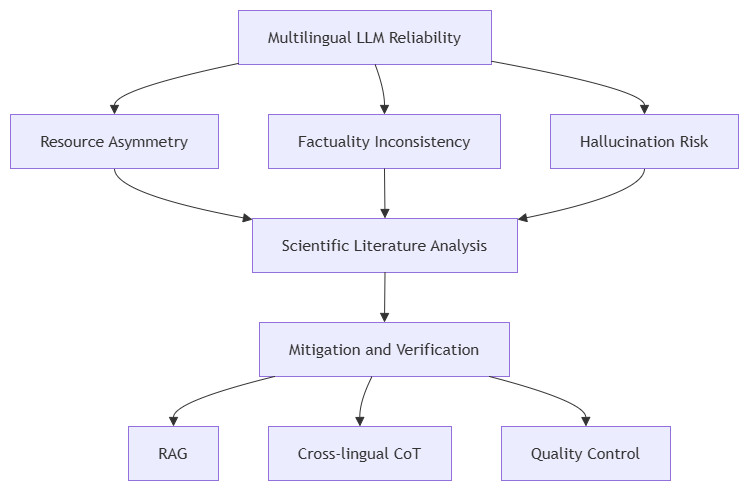
\includegraphics[
    width=\linewidth,
    keepaspectratio
]{Figures/conceptual_framework.png}

\caption{
Conceptual framework used in this review. Reliability is treated as an interaction among language/data conditions, evaluation design, generation and grounding mechanisms, and application-level quality control.
}

\Description{
Conceptual framework showing how multilingual reliability in LLM-based scientific literature analysis depends on interactions among language and data conditions, evaluation, generation and grounding, and application-level quality control.
}

\label{fig:taxonomy}

\end{figure}

% =========================================================
% 3. BACKGROUND AND RELATED WORK
% =========================================================

\section{Background and Related Work}
\label{sec:background}

% ---------------------------------------------------------
% 3.1
% ---------------------------------------------------------

\subsection{Multilingual Large Language Models}
\label{sec:multilingual-models}

The development of multilingual language models has expanded the number of languages that can be processed within a shared model. mT5 was pretrained on a Common Crawl-based corpus covering 101 languages and demonstrated multilingual transfer across several benchmarks \citep{xue2021mt5}. BLOOM extended this direction with a 176-billion-parameter open-access model trained on the ROOTS corpus, which contains material from 46 natural languages and 13 programming languages \citep{bigscience2022bloom}. GPT-4 also reports multilingual benchmark results, although its technical report does not establish uniform reliability across all languages or scientific domains \citep{openai2023gpt4}.

Multilingual coverage, however, does not imply equivalent capability. XTREME evaluates cross-lingual generalization across 40 languages and 9 tasks and reports substantial variation across languages and tasks \citep{hu2020xtreme}. MMLU-ProX extends parallel multilingual evaluation to 29 languages and reports marked differences between high-resource and low-resource languages \citep{xuan2025mmlupro}. Together, these studies motivate evaluating language-specific reliability rather than relying on a single aggregate multilingual score.

% ---------------------------------------------------------
% 3.2
% ---------------------------------------------------------

\subsection{LLMs for Scientific Literature Analysis}
\label{sec:lit-review-automation}

A growing research stream evaluates LLMs for components of literature-review workflows. Scherbakov et al. conducted a systematic review of LLM use in literature reviews and reported that GPT-based systems represented a large share of the reviewed applications, while performance varied by workflow stage \citep{scherbakov2025emergence}. Wu et al. developed an automated literature-research and review-generation system with layered quality-control procedures \citep{wu2025automated}. Tang et al. evaluated reference generation, abstract writing, and review composition using multidimensional metrics and found that advanced models could still generate hallucinated references and that performance varied across disciplines \citep{tang2025automated}.

An important limitation is that the evidence base for automated literature analysis remains concentrated on English-language material. Consequently, evidence about the multilingual reliability of these systems is less mature than evidence about general multilingual language-model capability.

% ---------------------------------------------------------
% 3.3
% ---------------------------------------------------------

\subsection{Cross-Lingual Factuality and Confidence}
\label{sec:factuality-background}

Qi et al. introduced Ranking-based Consistency (RankC) to study whether factual knowledge is represented consistently across languages. Their analysis found that increasing model size improved factual probing accuracy in many languages but did not necessarily improve cross-lingual consistency \citep{qi2023crosslingual}. This distinction is important for literature analysis because a model can answer correctly in one language while producing a different factual response to an equivalent query in another language.

Xue et al.'s MlingConf study further shows that confidence estimation can exhibit language dominance effects. Their results indicate that language-specific prompting can improve confidence-estimation behavior for some language-specific tasks \citep{xue2024mlingconf}. Together, these studies suggest that multilingual reliability should include not only accuracy but also consistency and calibration.

% =========================================================
% 4. MULTILINGUAL RELIABILITY
% =========================================================

\section{Multilingual Reliability in Scientific Literature Analysis}
\label{sec:reliability}

% ---------------------------------------------------------
% 4.1
% ---------------------------------------------------------

\subsection{Cross-Lingual Performance and Resource Asymmetry}
\label{sec:resource-asymmetry}

The reviewed benchmarks consistently indicate that multilingual performance is heterogeneous. XTREME demonstrated cross-language differences across a broad set of tasks \citep{hu2020xtreme}, while MMLU-ProX reports marked performance disparities across its 29-language evaluation setting \citep{xuan2025mmlupro}. These results are not direct measurements of scientific literature analysis, but they establish a relevant baseline: language-resource level can affect the reliability of downstream reasoning and information processing.

For scientific applications, the resource issue can compound with domain specialization. Scientific terminology, named entities, abbreviations, and methodological descriptions may be sparsely represented in non-English training and evaluation data. A model can therefore face simultaneous language-resource and domain-resource constraints. This motivates separating general language effects from scientific-domain effects in future evaluation designs.

% ---------------------------------------------------------
% 4.2
% ---------------------------------------------------------

\subsection{Factual Consistency Across Languages}
\label{sec:factual-consistency}

Cross-lingual factual inconsistency is particularly consequential for scientific use. If equivalent questions produce different factual answers depending on the language of the query, multilingual users may receive unequal access to the same scientific knowledge. Qi et al.'s RankC analysis provides evidence that factual knowledge is not uniformly aligned across languages and that knowledge inserted or edited in English may transfer unevenly to other languages \citep{qi2023crosslingual}.

For literature synthesis, this problem can appear at multiple points: query formulation, retrieval, extraction, translation, and final generation. Therefore, evaluating only the final answer can obscure the stage at which a reliability failure occurred.

% ---------------------------------------------------------
% 4.3
% ---------------------------------------------------------

\subsection{Hallucination and Citation Reliability}
\label{sec:hallucination}

Hallucination is a central reliability problem in automated literature review. Tang et al. explicitly evaluated hallucination in generated references and found that even advanced LLMs continued to produce hallucinated references \citep{tang2025automated}. Wu et al. demonstrated that layered verification can reduce citation-related hallucination in an automated review-generation setting \citep{wu2025automated}. These results support the use of verification rather than treating a fluent generated review as sufficient evidence.

The multilingual case introduces an additional dependency: verification requires searchable and interpretable source material in the target language. If retrieval indices, metadata, abstracts, or scientific corpora have weaker coverage for a language, the quality-control stage may inherit the same asymmetry as the generation stage.

% ---------------------------------------------------------
% 4.4
% ---------------------------------------------------------

\subsection{Domain-Specific Scientific and Biomedical Gaps}
\label{sec:domain-gaps}

Scientific and biomedical text introduces specialized terminology and entity relations that are not necessarily captured by general-purpose multilingual benchmarks. This creates a need for domain-specific evaluation rather than assuming that results on general knowledge benchmarks transfer directly to scientific literature analysis.

A useful conceptual distinction is therefore between \emph{language capability} and \emph{scientific reliability}. The former concerns whether a model can process a language; the latter additionally requires accurate handling of scientific terminology, claims, citations, numerical information, and source context.

% ---------------------------------------------------------
% 4.5
% ---------------------------------------------------------

\subsection{Confidence and Downstream Risk}
\label{sec:confidence-risk}

Confidence is relevant because users may use model certainty as a proxy for reliability. MlingConf reports language-dependent confidence behavior and shows that prompting in the query-related language can affect confidence estimation for language-specific tasks \citep{xue2024mlingconf}. In scientific workflows, incorrect but confident outputs can be especially problematic because they may be copied into notes, reports, or subsequent synthesis stages without adequate verification.

% =========================================================
% 5. CURRENT APPROACHES
% =========================================================

\section{Current Approaches and Developments}
\label{sec:approaches}

The main approaches identified in the literature are summarized in Table~\ref{tab:comparative}. No single approach addresses every source of multilingual reliability error; each operates at a different layer of the taxonomy in Figure~\ref{fig:taxonomy}.

% ---------------------------------------------------------
% COMPARATIVE TABLE
% ---------------------------------------------------------

\begin{table*}[t]

\caption{
Comparative synthesis of representative research relevant to multilingual reliability and LLM-assisted scientific literature analysis.
}

\label{tab:comparative}

\centering
\small

\begin{tabularx}{\textwidth}
{@{}p{0.15\textwidth}
 p{0.16\textwidth}
 p{0.18\textwidth}
 X
 p{0.18\textwidth}@{}}

\toprule

\textbf{Study}
&
\textbf{Focus}
&
\textbf{Data / Evaluation}
&
\textbf{Main contribution}
&
\textbf{Limitation relevant to this review}
\\

\midrule

Xue et al. \citep{xue2021mt5}
&
Multilingual pretraining
&
101 languages
&
Demonstrates large-scale multilingual text-to-text transfer
&
General multilingual capability does not by itself establish scientific reliability
\\

BigScience \citep{bigscience2022bloom}
&
Open multilingual LLM
&
46 natural languages + 13 programming languages
&
Provides an open large-scale multilingual model and multilingual training resource
&
Broad coverage does not imply uniform language or domain performance
\\

Hu et al. \citep{hu2020xtreme}
&
Cross-lingual benchmarking
&
40 languages, 9 tasks
&
Establishes systematic cross-lingual comparison
&
General NLP tasks are not specific to scientific literature analysis
\\

Qi et al. \citep{qi2023crosslingual}
&
Factual consistency
&
Multilingual factual probing; RankC
&
Shows that factual knowledge can be inconsistent across languages
&
Focuses on factual knowledge rather than complete literature-review pipelines
\\

Xue et al. \citep{xue2024mlingconf}
&
Confidence estimation
&
Multilingual confidence tasks
&
Identifies language-dominance effects in confidence estimation
&
Confidence is only one component of scientific reliability
\\

Scherbakov et al. \citep{scherbakov2025emergence}
&
Literature-review automation
&
Systematic review of LLM-assisted reviews
&
Maps how LLMs are being used across review workflows
&
Evidence base is dominated by English-language applications
\\

Wu et al. \citep{wu2025automated}
&
Automated review generation
&
343 articles across 35 topics
&
Demonstrates layered quality-control for automated review generation
&
Multilingual generalization is not established
\\

Tang et al. \citep{tang2025automated}
&
Review-generation evaluation
&
Reference generation, abstract writing, review composition
&
Measures hallucination, semantic coverage, and factual consistency
&
Evaluation remains primarily English-language and discipline-dependent
\\

Xuan et al. \citep{xuan2025mmlupro}
&
Multilingual reasoning benchmark
&
29 languages; parallel questions
&
Enables direct cross-lingual comparison and documents disparities
&
Not specifically designed for scientific literature workflows
\\

\bottomrule

\end{tabularx}

\end{table*}

% ---------------------------------------------------------
% 5.1 RAG
% ---------------------------------------------------------

\subsection{Retrieval-Augmented and Knowledge-Grounded Generation}
\label{sec:rag}

Retrieval-augmented generation (RAG) supplies source material at inference time so that generation can be grounded in retrieved evidence. For scientific literature analysis, retrieval can reduce dependence on parametric memory and make source verification more explicit. However, multilingual RAG inherits the coverage of its retrieval index: weak indexing, sparse metadata, or limited target-language scientific documents can reduce the quality of the evidence supplied to the model.

% ---------------------------------------------------------
% 5.2
% ---------------------------------------------------------

\subsection{Cross-Lingual Reasoning and Knowledge Transfer}
\label{sec:crosslingual-reasoning}

Cross-lingual reasoning methods attempt to use a high-resource language as an intermediate reasoning or knowledge-transfer channel. Such approaches are promising because they can exploit stronger model capabilities in high-resource languages, but they also introduce possible translation and semantic-alignment errors. Their evaluation should therefore measure both target-language output quality and preservation of scientific meaning.

% ---------------------------------------------------------
% 5.3
% ---------------------------------------------------------

\subsection{Multilingual and Domain-Specific Fine-Tuning}
\label{sec:finetuning}

Targeted fine-tuning can improve performance when high-quality domain data are available. The broader multilingual-model literature suggests that data quality and language coverage remain important constraints \citep{xue2021mt5,bigscience2022bloom}. For scientific applications, domain-specific adaptation should be evaluated against general multilingual models using the same scientific tasks and languages.

% ---------------------------------------------------------
% 5.4
% ---------------------------------------------------------

\subsection{Multilayered Quality Control}
\label{sec:quality-control}

Application-level quality control can combine source retrieval, citation checking, consistency checks, and expert review. Wu et al. provide an example of a layered automated review-generation pipeline \citep{wu2025automated}, while Tang et al. show why reference generation and review composition require explicit evaluation rather than assuming that model fluency implies factual correctness \citep{tang2025automated}. For multilingual systems, these controls should operate on the original-language sources as well as translated representations.

% =========================================================
% 6. RESEARCH CHALLENGES
% =========================================================

\section{Research Challenges and Limitations}
\label{sec:challenges}

% ---------------------------------------------------------
% 6.1
% ---------------------------------------------------------

\subsection{Scarcity of Non-English Scientific Corpora}
\label{sec:corpora}

A recurring limitation is the scarcity of large, high-quality scientific corpora and annotations outside English. This affects both model adaptation and evaluation. Without representative target-language scientific data, it is difficult to determine whether an observed error is caused by language-resource scarcity, domain scarcity, or model behavior.

% ---------------------------------------------------------
% 6.2
% ---------------------------------------------------------

\subsection{Translation Artifacts in Benchmark Construction}
\label{sec:translation}

MMLU-ProX illustrates both the value and difficulty of constructing parallel multilingual benchmarks. Its language versions are built through translation followed by expert review \citep{xuan2025mmlupro}. Such procedures improve scalability, but benchmark construction can still introduce translation-specific artifacts that do not occur in naturally authored scientific texts.

% ---------------------------------------------------------
% 6.3
% ---------------------------------------------------------

\subsection{Language--Domain Confounding}
\label{sec:confounding}

A model may perform poorly on a scientific query because the language is underrepresented, because the scientific subdomain is underrepresented, or because both factors interact. Existing benchmarks do not always separate these variables. Future experiments should therefore use factorial or matched designs that vary language resource level and domain coverage independently.

% ---------------------------------------------------------
% 6.4
% ---------------------------------------------------------

\subsection{Absence of a Standardized Scientific-Reliability Benchmark}
\label{sec:metrics}

General multilingual benchmarks such as XTREME and MMLU-ProX provide important infrastructure, but they do not directly measure all requirements of scientific literature analysis. A dedicated benchmark should include claim verification, citation grounding, numerical fidelity, methodological summarization, evidence completeness, and cross-lingual consistency.

% ---------------------------------------------------------
% 6.5
% ---------------------------------------------------------

\subsection{English-Centric Evidence Base}
\label{sec:english-bias}

The evidence base for LLM-assisted literature analysis remains substantially English-centric. This creates a methodological limitation in the literature itself: conclusions about the reliability of automated review systems may be based on a narrower linguistic population than the systems' intended user base.

% =========================================================
% 7. RESEARCH GAPS AND FUTURE DIRECTIONS
% =========================================================

\section{Research Gaps and Future Directions}
\label{sec:gaps}

% ---------------------------------------------------------
% 7.1
% ---------------------------------------------------------

\subsection{Multilingual Scientific-Reliability Benchmarks}
\label{sec:benchmark-gap}

Future benchmarks should combine the parallel-comparison principle of MMLU-ProX with scientific tasks such as claim verification, citation grounding, evidence extraction, and methodological summarization \citep{xuan2025mmlupro}. Expert validation should be performed independently of the LLMs used to construct or translate benchmark items.

% ---------------------------------------------------------
% 7.2
% ---------------------------------------------------------

\subsection{Non-English Scientific Corpora and Annotation Infrastructure}
\label{sec:corpus-gap}

The field needs curated scientific corpora across languages and disciplines, together with annotations for claims, entities, relations, citations, and evidence spans. Such resources would allow evaluation to move beyond translated general-purpose benchmarks toward naturally authored scientific material.

% ---------------------------------------------------------
% 7.3
% ---------------------------------------------------------

\subsection{Disentangling Language and Domain Effects}
\label{sec:disentangle-gap}

Evaluation should explicitly separate language-resource effects from domain-specific effects. One useful design is to evaluate the same scientific task across several languages while holding the domain constant, and then repeat the experiment across several scientific domains within the same language.

% ---------------------------------------------------------
% 7.4
% ---------------------------------------------------------

\subsection{Cross-Lingual Verification and Grounding}
\label{sec:verification-gap}

Future literature-review systems should combine multilingual retrieval with source-grounded generation and automated verification. Evaluation should report not only final-answer accuracy but also retrieval recall, citation correctness, evidence alignment, and the preservation of scientific meaning through translation or cross-lingual reasoning.

% ---------------------------------------------------------
% 7.5
% ---------------------------------------------------------

\subsection{Transparent Reporting of Language Coverage}
\label{sec:reporting-gap}

LLM-assisted review studies should report the languages represented in their source corpus, retrieval index, prompts, evaluation set, and verification process. This would make it easier to determine whether a reported reliability result applies to multilingual scientific use or only to an English-centered setting.

% ---------------------------------------------------------
% 7.6 EQUATION
% ---------------------------------------------------------

\subsection{A Reliability-Gap Measure}
\label{sec:gap-measure}

For studies that compare language-resource groups using a common reliability metric, the gap can be expressed as

\begin{equation}
\Delta R = R_{\mathrm{high}} - R_{\mathrm{low}}
\label{eq:reliability-gap}
\end{equation}

where $R_{\mathrm{high}}$ and $R_{\mathrm{low}}$ denote reliability measurements for higher-resource and lower-resource language groups, respectively. Equation~\ref{eq:reliability-gap} is a descriptive difference, not a universal metric: studies must define the underlying reliability measure and evaluation population explicitly.

% ---------------------------------------------------------
% RESEARCH GAPS TABLE
% ---------------------------------------------------------

\begin{table}[t]

\caption{Research gaps and corresponding directions.}

\label{tab:research-gaps}

\centering

\small

\begin{tabularx}{\linewidth}
{@{}p{0.31\linewidth}X@{}}

\toprule

\textbf{Observed gap}
&
\textbf{Future direction}
\\

\midrule

Sparse non-English scientific data
&
Build naturally authored multilingual scientific corpora and expert annotations.
\\

No dedicated scientific-reliability benchmark
&
Evaluate claim verification, citation grounding, numerical fidelity, and methodological summarization across languages.
\\

Language/domain confounding
&
Use matched experiments that vary language resource level and scientific domain independently.
\\

Weak multilingual verification infrastructure
&
Combine multilingual retrieval, source-grounded generation, and automated citation/evidence checks.
\\

Limited reporting of language coverage
&
Require explicit reporting of source, retrieval, prompt, evaluation, and verification languages.
\\

\bottomrule

\end{tabularx}

\end{table}

% =========================================================
% 8. CONCLUSION
% =========================================================

\section{Conclusion}
\label{sec:conclusion}

The reviewed literature indicates that multilingual LLM capability is heterogeneous rather than uniform. Multilingual benchmarks demonstrate meaningful variation across languages, cross-lingual factuality research shows that knowledge can be represented inconsistently, and recent literature-review evaluations show that hallucinated references and factual errors remain relevant even for advanced models \citep{hu2020xtreme,qi2023crosslingual,xuan2025mmlupro,tang2025automated}. These findings are important for scientific literature analysis because errors can propagate across retrieval, extraction, translation, synthesis, and citation stages.
Current mitigation approaches---including retrieval augmentation, cross-lingual reasoning, multilingual/domain-specific adaptation, and multilayered verification---address different parts of the reliability problem. Their benefits should therefore be evaluated with stage-specific and language-specific metrics rather than a single overall score. In particular, multilingual scientific reliability cannot be inferred solely from general-purpose benchmark performance.

The main research opportunity is to develop evaluation and infrastructure that treat language coverage as a first-class scientific variable. Expert-validated multilingual scientific benchmarks, naturally authored non-English scientific corpora, matched language/domain experiments, source-grounded multilingual retrieval, and transparent reporting can provide a stronger basis for evaluating whether LLM-assisted literature analysis is reliable across languages. Such work would also make it possible to distinguish improvements in general multilingual capability from improvements that specifically benefit scientific evidence synthesis.

% =========================================================
% REFERENCES
% =========================================================

\bibliographystyle{ACM-Reference-Format}

\bibliography{references}

\end{document}